% .latexmkrc resolves this class from the official template supplied with the
% project under ../IEEE-conference-template-062824/.
\documentclass[conference]{IEEEtran}

\usepackage{cite}
\usepackage{amsmath,amssymb,amsfonts}
\usepackage{algorithmic}
\usepackage{graphicx}
\usepackage{textcomp}
\usepackage[T1]{fontenc}
\usepackage{microtype}
\usepackage{xcolor}
\usepackage[hidelinks]{hyperref}
\usepackage{tikz}
\usetikzlibrary{arrows.meta,positioning}

\title{Regional English Accent Robustness in Direct and Cascaded
Speech-to-Text Translation: A Literature Survey}

\author{\IEEEauthorblockN{1\textsuperscript{st} Nathan Naylin}
\IEEEauthorblockA{\textit{Dept. of Science} \\
\textit{University of Auckland}\\
Auckland, New Zealand \\
nhte538@aucklanduni.ac.nz}
\and
\IEEEauthorblockN{2\textsuperscript{nd} Zhitong Li}
\IEEEauthorblockA{\textit{Dept. of Science} \\
\textit{University of Auckland}\\
Auckland, New Zealand \\
zli262@aucklanduni.ac.nz}
\and
\IEEEauthorblockN{3\textsuperscript{rd} Arizona Xing}
\IEEEauthorblockA{\textit{Dept. of Science} \\
\textit{University of Auckland}\\
Auckland, New Zealand \\
lxin541@aucklanduni.ac.nz}
\and
\IEEEauthorblockN{4\textsuperscript{th} Patricia Jennesha}
\IEEEauthorblockA{\textit{Dept. of Science} \\
\textit{University of Auckland}\\
Auckland, New Zealand \\
pjen088@aucklanduni.ac.nz}
\and
\IEEEauthorblockN{5\textsuperscript{th} Jidni Mayukh}
\IEEEauthorblockA{\textit{Dept. of Science} \\
\textit{University of Auckland}\\
Auckland, New Zealand \\
jmay830@aucklanduni.ac.nz}
}

\begin{document}

\maketitle

\begin{abstract}
Regional English accent is a source of uneven automatic speech
recognition performance, but its effect on final speech-translation quality is
less clearly established. This survey examines how accent may affect Direct
speech translation, which maps speech to translated text without an exposed
transcript, and Cascaded speech translation, which connects speech recognition
to machine translation. Twenty-seven works were retained through thematic
selection covering system architectures, accent robustness, error
propagation, datasets, translation metrics, and statistical comparison. The
review finds that neither architecture is consistently superior: reported
outcomes vary with language pair, training resources, test data, references,
and metrics. Accent-related recognition disparities are well established, and
recognition errors can damage downstream translation, but these findings do
not alone demonstrate accent-related translation degradation. The closest
speech-translation studies either lack controlled regional-accent labels, omit
a matched Cascaded comparator, or evaluate an adjacent downstream task.
Common Voice and CoVoST 2 enable a relevant evaluation, although self-reported
accent labels, repeated content, speaker dependence, and reference design
constrain interpretation. The gap is a matched evaluation of Direct
and Cascaded systems on the same regional-English utterances using final
translation quality, motivating the question: how does regional English accent
affect the translation quality of these two system categories?
\end{abstract}

\begin{IEEEkeywords}
speech translation, regional English accents, robustness, direct speech
translation, cascaded speech translation, automatic speech recognition
\end{IEEEkeywords}

\section{Introduction}
\label{sec:introduction}

This survey examines regional English accent as an important factor in
speech-to-text translation. It focuses on two main system types: Direct speech
translation (Direct ST) and Cascaded speech translation (Cascaded ST). Direct
ST translates source-language speech directly into target-language text
without producing an intermediate transcript. Cascaded ST first uses automatic
speech recognition (ASR) to convert speech into text and then applies machine
translation (MT) to produce the target-language translation. These two
approaches are compared throughout the survey, without assuming that either
one is always more accurate or more robust.

The survey is guided by the following research question:
\begin{quote}
\emph{How does regional English accent affect the translation quality of
Direct and Cascaded speech-to-text translation systems?}
\end{quote}
The main focus is final translation quality across regional accent groups.
Word error rate (WER) is considered only as a diagnostic measure for the ASR
stage of the Cascaded system. It is not treated as a direct measure of
translation quality.

The comparison is important because Direct and Cascaded systems have different
possible failure points. Cascaded systems can benefit from mature ASR and MT
models and from the larger datasets available for these separate tasks.
However, errors in the ASR transcript can be passed to the MT stage. Direct
systems remove this intermediate transcript, but they depend more strongly on
paired speech--translation data \cite{sperber2020endtoend}. Existing
comparisons do not show that one system type is always better. Results vary
depending on language pair, training resources, test segmentation, reference
translations, and evaluation metrics
\cite{bentivogli2021cascade,anastasopoulos2021iwslt,
etchegoyhen2022casestudy}. Therefore, overall system performance does not
directly show whether one approach is more robust to a particular regional
accent.

Accent is an important evaluation factor because ASR performance is not equal
across English varieties. Previous studies have reported performance
differences across regional, dialectal, and second-language accents, including
poorer performance on accents that were not represented during training
\cite{dichristofano2022global,jahan2025unveiling,shi2021aesrc,
prabhu2023accentcodebooks}. However, these findings mainly show an ASR-level
problem rather than a final translation result. This distinction is important
because similar WER values can lead to different levels of translation error,
while Direct ST does not produce an intermediate transcript where WER can be
measured \cite{le2017disentangling}. Previous work also shows that phonetic
recognition errors can reduce translation quality in Cascaded systems
\cite{sperber2019,pida2026}. This makes an accent effect on translation
plausible, but such an effect must still be measured using final translations
rather than inferred from ASR scores alone.

The literature was selected by theme rather than organised as a paper-by-paper
catalogue. The search covered Direct and Cascaded ST, ASR-to-MT error
propagation, accented ASR, unseen-accent generalisation, accented or dialectal
speech translation, accent-labelled datasets, speech-translation datasets,
evaluation metrics, and statistical reliability. Candidate papers and
publication details were checked through official sources, including ACL
Anthology, ISCA Archive, and IEEE proceedings. ArXiv papers were included when
no published venue version was identified. A paper was retained when its full
text had been reviewed and it directly contributed to at least one theme,
system comparison, evaluation issue, or test of the proposed research gap.
Blogs, secondary summaries, duplicate sources, and papers without verifiable
support for the required claims were excluded.

This process retained 27 studies, including recent work and older foundational
papers on evaluation metrics. Because a common systematic search record was
not maintained across all contributors, the survey is treated as a focused
narrative literature survey rather than an exhaustive systematic review.

The survey makes three main contributions. First, it connects research on
Direct and Cascaded speech translation with research on accent-sensitive ASR,
while keeping ASR error and translation quality as separate concepts. Second,
it examines whether the proposed research gap has already been addressed by
the closest studies on accent robustness, speech translation, and error
propagation. Third, it identifies the dataset, reference, metric, and
statistical controls needed for a fair comparison of final translation quality
across regional accent groups.

The remainder of the survey is organised as follows. Section
\ref{sec:architectures} reviews Direct and Cascaded speech-translation systems
and their empirical comparisons. Section~\ref{sec:accent-asr} examines accent
robustness in ASR. Section~\ref{sec:accent-st} reviews work that connects
accent, error propagation, and speech translation. Section~\ref{sec:evaluation}
discusses datasets, reference quality, evaluation metrics, and statistical
reliability. Section~\ref{sec:synthesis} combines the findings across these
themes to assess the research gap. Finally, Section~\ref{sec:conclusion}
presents the conclusion and the research question supported by the literature.

\section{Speech Translation Architectures and System Comparisons}
\label{sec:architectures}

\subsection{Architectures: Direct vs. Cascaded Paradigms}

\begin{figure}[!ht]
\centering
\resizebox{\columnwidth}{!}{%
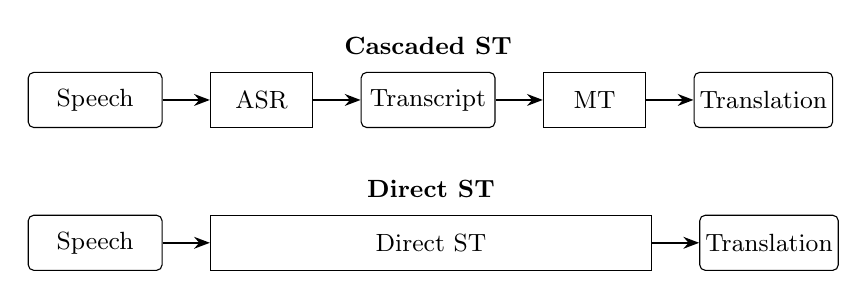
\begin{tikzpicture}[
  node distance=6mm and 6mm,
  data/.style={draw, rounded corners=2pt, minimum height=7mm,
    minimum width=17mm, align=center, font=\small, inner sep=2pt},
  proc/.style={draw, minimum height=7mm, minimum width=13mm,
    align=center, font=\small, inner sep=2pt},
  lbl/.style={font=\small\bfseries},
  arrow/.style={-{Stealth[length=2mm]}, thick}
]

% Cascaded pipeline
\node[data] (audio1) {Speech};
\node[proc, right=of audio1] (asr) {ASR};
\node[data, right=of asr] (text) {Transcript};
\node[proc, right=of text] (mt) {MT};
\node[data, right=of mt] (trans1) {Translation};

\draw[arrow] (audio1) -- (asr);
\draw[arrow] (asr) -- (text);
\draw[arrow] (text) -- (mt);
\draw[arrow] (mt) -- (trans1);

\node[lbl, above=1mm of text] {Cascaded ST};

% Direct pipeline
\node[data, below=11mm of audio1] (audio2) {Speech};
\node[proc, right=of audio2, minimum width=56mm] (direct)
  {Direct ST};
\node[data, right=of direct] (trans2) {Translation};

\draw[arrow] (audio2) -- (direct);
\draw[arrow] (direct) -- (trans2);

\node[lbl, above=1mm of direct] {Direct ST};

\end{tikzpicture}%
}
\caption{Simplified inference pipelines based on Sperber and
Paulik~\cite{sperber2020endtoend}. The cascade passes a single best
source-language transcript from ASR to MT. Direct ST produces target-language
text without an intermediate transcript.}
\label{fig:cascade-direct}
\end{figure}

Cascaded speech translation (ST) works as a two-step pipeline. An automatic
speech recognition (ASR) module first transcribes the audio into text in the
source language, and a machine translation (MT) model then translates that
transcript into the target language. The advantage of this separation is
practical. The two components can be developed, trained and replaced
independently. Each can also use the corpora already collected for its own
task: ASR draws on speech paired with transcripts, MT on parallel text, and
both are more widely available than audio paired with
translations~\cite{sperber2020endtoend}. Fig.~\ref{fig:cascade-direct}
contrasts this pipeline with the direct alternative described below.

The same separation creates the weakness most often associated with this
design: error propagation. Where the interface between the two components is
a single best transcript, recognition errors can pass into the MT stage, and
the MT model cannot return to the acoustic signal to check what was said.
The size of this effect varies. Le et al.~\cite{le2017disentangling} studied
French-to-English speech translation and found that improving the ASR
component from 21.86\% to 16.90\% word error rate on their development set
raised BLEU from 26.73 to 28.89. A few recognition errors sometimes caused
many translation errors, whereas a larger number, including morphological
substitutions, could have little effect. Word error rate alone therefore
does not show how much recognition errors affect translation quality,
although their pipeline used phrase-based statistical MT and these effects
need not carry over to neural systems.

Error propagation can be reduced. Sperber and
Paulik~\cite{sperber2020endtoend} list lattices, confusion networks and
error-tolerant MT as established countermeasures, and the cascade of Bentivogli
et al.~\cite{bentivogli2021cascade} fine-tunes its MT component on a mixture of
human and automatic transcripts for the same reason. Two other problems arise
at the interface between the components. MT models trained mainly on written
text may struggle with the disfluent, spoken-style output that ASR produces, a
mismatch between MT training text and ASR output. And once the pipeline commits
to a transcript, anything the transcript does not encode, including prosody, is
lost to the MT model~\cite{sperber2020endtoend}.

Direct ST architectures bypass the intermediate transcript. Weiss et
al.~\cite{weiss2017sequence} built an early direct sequence-to-sequence
system of this kind on 163 hours of Spanish telephone speech paired with
English translations, mapping acoustic features onto target-language text in
a single network. Removing the transcript interface removes the error
propagation that comes with it, and a single model can in principle run with
lower latency than two chained models, although Weiss et al. did not report
latency measurements. Paired speech and translation data is scarce, and
harder to obtain than the separate ASR and MT corpora available to cascaded
systems. Sperber and Paulik~\cite{sperber2020endtoend} describe this as a
possible trade-off between data efficiency and modelling power, and note
that the techniques direct models use to compensate, such as training on ASR
and MT data, may reintroduce some of the issues associated with cascades.
They present this as a question for further analysis rather than a settled
result.

\subsection{Empirical System Comparisons}

Bentivogli et al.~\cite{bentivogli2021cascade} compared cascaded and direct
systems built on the same core Transformer technology, drawing on overlapping
training resources used through different pipelines, and evaluated both on the
same MuST-C test segments for English to German, Spanish and Italian. They used
automatic metrics together with professional post-editing, assessed using two
measures based on translation edit rate (TER): human-targeted TER (HTER) and
multi-reference TER (mTER). On those post-editing measures the two approaches
performed similarly for English-to-German and English-to-Italian. For
English-to-Spanish the direct system was significantly better, while BLEU
computed against independent references favoured the cascade. The authors note
that these measures can lead to different conclusions.

A more detailed analysis showed different error patterns across directions. The
cascade made fewer morphological errors in English-to-German and
English-to-Italian, and fewer word-order errors in English-to-German. For
English-to-Spanish, the direct system made fewer lexical, morphological and
word-order errors. On a filtered subset prepared for manual annotation, direct
systems left more source words untranslated, though some omissions were
discourse markers that the authors say need not count as errors. The direct
system appeared to handle prosody better and made fewer errors in understanding
speech. The authors call both findings tentative, since few prosody cases could
be isolated and errors inside direct models are harder to observe.

The direct model used an encoder initialised from an ASR model, knowledge
distillation from a teacher MT model, and synthetic data produced by translating
transcripts from ASR training corpora~\cite{bentivogli2021cascade}. The
experiment therefore does not show that a direct model could match the cascade
without ASR and MT resources, nor that the gains it does achieve follow from
the inference architecture alone.

A study of Basque and Spanish reported different results. Etchegoyhen et
al.~\cite{etchegoyhen2022casestudy} compared both directions for this pair,
where Basque has rich morphology and relatively free word order. On their
main test sets the cascade was stronger for Basque-to-Spanish, while a
wav2vec-based direct model scored higher for Spanish-to-Basque. In a manual
ranking on a separate sample of parliamentary speech, evaluators preferred
the cascaded output in every configuration except Spanish-to-Basque with
additional training data, where the two were judged roughly equal. When
results were grouped by ASR word error rate, direct models did not
consistently perform better on subsets with higher WER. The pattern varied
with language direction and training data.

Shared tasks compare more systems, which differ in many respects besides
architecture. In the IWSLT 2021 offline task, cascaded systems took the top two
places, and the best cascade scored 2 BLEU points above the best direct
submission. With the original subtitle-style TED references, a different direct
submission ranked highest among direct systems, and the gap to the best cascade
was 0.7 BLEU. This shows that reference choice can change both system rankings
and the apparent gap between the two approaches. In the multilingual task of
the same campaign, the three teams submitting both architectures found their
direct systems stronger.
The organisers suggest that differences between the tasks in auxiliary data
volume and in audio segmentation may help explain
this~\cite{anastasopoulos2021iwslt}. Two years later, cascaded systems were
again generally stronger in the IWSLT 2023 offline
task~\cite{agarwal2023iwslt}.

More recently, Papi et al.~\cite{papi2026hearing} benchmarked twenty-two
systems, four direct and twelve cascaded alongside six speech-enabled language
models, across sixteen benchmarks and a range of acoustic and linguistic
conditions. Cascaded systems were the most reliable overall, and performance
depended on the condition tested rather than on the architecture alone. In a
human evaluation comparing one model from each group, the direct model produced
more undertranslation than the cascade, consistent with the pattern reported by
Bentivogli et al.~\cite{bentivogli2021cascade}.

\subsection{From System Comparisons to Accent}

Across these studies, no approach performs best in every setting, and the
reported differences vary with the language pair, the evaluation data, the
reference translations and the metric, a dependence examined further in
Section~\ref{sec:evaluation}. Earlier comparisons such as Bentivogli et
al.~\cite{bentivogli2021cascade} and Etchegoyhen et
al.~\cite{etchegoyhen2022casestudy} did not report results by accent group.
Other speech conditions were also considered: Weiss et
al.~\cite{weiss2017sequence} used telephone speech, and Bentivogli et
al.~\cite{bentivogli2021cascade} analysed audio duration and speech rate and
examined errors involving poor audio quality or overlapping speech.

Recent studies report accent-level results. The IWSLT 2024 offline task
added an accent challenge built from the Edinburgh International Accents of
English Corpus, and all submissions to that task used a cascaded
architecture~\cite{ahmad2024iwslt}. Papi et al.~\cite{papi2026hearing}
evaluate accent conditions across direct, cascaded and speech-enabled
systems and suggest that the choice of speech encoder matters for accent
robustness. Section~\ref{sec:accent-st} examines accent robustness in speech
translation in more detail. Comparisons at the system level can show how
translation quality varies across accent groups, but they do not on their
own explain where those differences come from. The next section reviews how
accent affects ASR, which may help explain errors in cascaded speech
translation.

\section{Accent Robustness in Speech Processing}
\label{sec:accent-asr}

% TODO(Member 2): Owner: Member 2. Target approximately 1.7 pages.
% Purpose: synthesize evidence on regional/accented English ASR, including
% seen versus unseen accents, underrepresented groups, generalization,
% adaptation, and limitations.
% Evidence needed: approximately five personally read peer-reviewed papers.
% Comparisons needed: accent definitions, speaker-disjoint evaluation,
% training/test overlap, dataset balance, WER patterns, adaptation trade-offs,
% and which populations are missing or aggregated.
% Boundary: this section may establish accent sensitivity in ASR but must not
% present ASR WER as direct evidence of final translation quality.
% Transition in: explain why architecture evidence must be paired with speech
% variation evidence.
% Transition out: make explicit which ASR findings motivate, but do not answer,
% the speech-translation question in Section IV.
\collabplaceholder{Member 2}{Develop the accent-ASR synthesis using verified
sources. Compare datasets, evaluation conditions, generalization, adaptation,
strengths, and limitations, while preserving the boundary between recognition
and final translation evidence.}

\section{Accent Robustness in Speech Translation}
\label{sec:accent-st}

Section III established that accent-related degradation in automatic speech recognition (ASR) is systematic, measurable, and present across the open model families relevant to this project, including Whisper and SeamlessM4T. That evidence, however, is confined to ASR-level metrics such as word error rate (WER) and word information lost (WIL). It does not by itself establish whether accent-driven recognition error affects final translation quality, or whether the two architectural paradigms compared in this survey are affected to a similar degree. This section reviews work at the intersection of accent, error propagation, and speech translation (ST) to test whether that specific combination has already been addressed.

One important area of research concerns the effect of ASR errors on cascaded ST. Sperber \textit{et al.} \cite{sperber2019} investigated this by directly manipulating the intermediate ASR transcripts provided to different translation systems. They compared systems using correct reference transcripts, normal ASR output, and transcripts containing artificially introduced substitution, insertion, and deletion noise. They report that the cascade responds most strongly to both improved and degraded labels, confirming that it is the architecture most exposed to intermediate transcription error, while models with continuous access to acoustic information are comparatively, though not completely, insulated.

Nguyen \textit{et al.} \cite{pida2026} quantify this effect directly for Vietnamese-English cascaded ST, reporting BLEU drops of 6.79 to 10.64 points when translating ASR output rather than clean reference transcripts. Using linear mixed-effects modelling, they further show that, among substitution-type errors specifically, most arise from a systematic phonetic cause involving vowels, consonants, and tones rather than from phonetically unrelated substitutions. The phonetic-confusion categories are statistically significant predictors of translation-quality degradation, whereas phonetically unrelated substitutions are not. Insertions and deletions, however, remain the largest-magnitude predictors of translation-quality degradation overall. Read together with the AESRC2020 and accent-codebook evidence from Section III, this is a relevant methodological bridge: if accent variation is itself a phonetically systematic source of ASR error, and phonetically systematic substitution errors are significant (if not the largest-magnitude) contributors to cascaded translation-quality loss, then the mechanism by which accent could degrade cascaded ST specifically is plausible and consistent with existing evidence, even though neither study manipulates accent as an independent variable.

A second group of studies examines the robustness of speech models to other forms of variation. The SeamlessM4T technical report \cite{seamlessm4t2023} and its successor \cite{seamless2023} benchmark robustness to background noise and to what the authors label ``speaker variations'' or ``vocal style variations,'' reporting that SeamlessM4T outperforms a Whisper-Large-v2 baseline by a substantial margin on both axes, using BLEU/chrF-based metrics and a coefficient-of-variation measure across speaking styles. This is the closest published evidence to a controlled Direct-versus-Whisper robustness comparison among the model families used in this project. Two limitations constrain how far it can be read as evidence for the present research question. First, ``speaker variation'' in these reports is not equivalent to, and is not reported as, regional accent; the test conditions are not accent-labelled, so any accent effect is at best a subset of an unspecified broader category. Second, the comparison evaluates Whisper alone rather than a full Whisper-to-MT cascade of the kind this project benchmarks, so a cascade-specific error-propagation effect of the kind documented by Sperber \textit{et al.} is not isolated in these results. The reported robustness advantage of SeamlessM4T over Whisper therefore cannot be attributed to accent specifically, nor to the direct-versus-cascade distinction as operationalised in this survey.

A narrower but genuinely relevant example comes from Havare \textit{et al.} \cite{losttranscription2026}, who study a multilingual, code-mixed speech-driven framework for programming queries. In their qualitative failure-mode taxonomy, the authors explicitly name ``accent based errors'' as one of seven ASR failure modes, giving concrete regional examples: ``default'' pronounced with a Marathi accent is transcribed as ``de fall,'' and ``machine'' pronounced with a Telugu accent becomes ``mishan.'' This is the clearest example identified in this survey of accent named explicitly, with concrete regional examples, as a cause of ASR misrecognition within a multi-stage pipeline. The paper also quantifies downstream propagation directly: on a code-retrieval task, Recall@5 drops from 92\% using gold-text queries to 87\% using raw ASR-transcribed queries, and MRR drops from 87.2\% to 81.58\%, before an LLM-based correction stage partially recovers performance. Two limitations nonetheless constrain how far this can be read as evidence for the present research question. First, the accent-based failure mode is presented qualitatively, with two illustrative examples, rather than as a controlled variable in the paper's quantitative evaluation. The reported WER, PER, WFED, and Recall/MRR results are instead broken down by target language, not by accent group. Therefore, the quantified downstream-degradation numbers cannot themselves be attributed to accent specifically. Second, the domain is code-mixed spoken programming queries processed through a Whisper/Indic-Conformer ASR stage feeding an LLM-based retrieval pipeline, not natural spoken-English translation compared across a Direct-versus-Cascaded ST architecture; no direct-style architecture is evaluated as a comparator in the sense used in this survey. The paper is therefore genuine, if partial, evidence that accent-driven ASR error can propagate into degraded downstream task performance in at least one adjacent pipeline, but it does not establish this for speech translation specifically, nor for a Direct-versus-Cascaded comparison.

Read together, these strands of literature support two provisional conclusions. First, the mechanism through which accent-related ASR errors could affect cascaded translation quality is consistent with existing evidence. Error propagation in cascaded ST has been directly demonstrated, and phonetically systematic substitution errors have been shown to contribute significantly to translation-quality degradation. The evidence reviewed in Section III further establishes accent variation as a potential source of systematic phonetic differences, while Havare \textit{et al.} \cite{losttranscription2026} explicitly identify accent-related ASR errors and demonstrate their propagation into measurable downstream task degradation in an adjacent speech-processing application. The existing literature therefore provides a plausible theoretical and empirical basis for investigating accent-related degradation in cascaded ST. Second, no study identified in this survey evaluates matched Direct and Cascaded ST systems on the same accent-labelled regional English speech, using final translation quality as the outcome, with accent treated as a controlled rather than illustrative variable. The closest available architecture-level robustness comparison \cite{seamlessm4t2023,seamless2023} does not use accent-labelled data or a matched cascade condition, and the closest available accent-explicit propagation evidence \cite{losttranscription2026} names accent only qualitatively and outside the speech-translation domain. The combination of these elements, namely accent as a controlled variable, a matched Direct/Cascaded ST comparison, and final translation quality as the outcome, therefore represents a potential research gap. This gap must, however, be considered alongside the remaining themes reviewed in Section V before it can be established as the central research gap of the project.

\section{Evaluation Data and Methodological Evidence}
\label{sec:evaluation}

This section synthesizes the literature that determines how evidence about
accent and speech translation can be interpreted. It first examines dataset
and reference design, then considers translation metrics and statistical
reliability. Together, these themes establish the controls required for a
credible comparison without turning the survey into an experimental procedure.

\subsection{Accent-Labelled Speech Data}

Common Voice provides a practical source of accent-labelled speech, but the
status of those labels needs to be stated carefully. Ardila et al. describe
\texttt{accent} as one of three optional demographic fields self-reported by
speakers, alongside age and gender; the paper does not report expert phonetic
verification of this field \cite{ardila2020commonvoice}. Prabhu et al. later
extract an English validated subset, \texttt{MCV\_ACCENT}, and organize 14
Common Voice accent categories into five seen accents used for training and
validation and nine unseen accents used for testing. Their train, development,
and test sets are speaker-disjoint \cite{prabhu2023accentcodebooks}. This work
demonstrates that Common Voice metadata can support controlled
accent-robustness experiments, but neither paper establishes independent
validation of the accent categories. A version caveat is also necessary:
Ardila et al. describe Common Voice data from 2019, whereas Prabhu et al. do
not report the exact Common Voice release used for \texttt{MCV\_ACCENT}; their
counts and split details therefore should not be treated as describing an
identical dataset snapshot.

\subsection{Speech-Translation Data and Reference Quality}

CoVoST 2 supplies the translation layer that Common Voice itself lacks. Wang
et al. derive it from validated Common Voice read speech and send deduplicated
source transcripts, without the corresponding audio, to professional
translators \cite{wang2021covost2}. Translation quality is checked using
language-model perplexity, LASER scores, and a length-ratio heuristic.
Low-scoring items are manually inspected and retranslated, while sentences
that cannot be translated properly, often because of missing context, are
marked in the release. This process provides documented professional
translation and quality-control provenance. The paper also reports cascaded
and end-to-end ST baselines on the corpus; its end-to-end ST category
corresponds to the Direct ST category used in this survey
\cite{wang2021covost2}. However, the references are conditioned on text rather
than audio, and the authors warn that the CoVoST multi-speaker development and
test splits contain repeated sentences that may skew BLEU or WER. These
properties must therefore be considered when designing a comparable
evaluation.

\subsection{Dataset Design for Controlled Accent Comparisons}

Together, the three papers show that a fair comparison between Direct and
Cascaded ST requires careful control of the evaluation data. Common Voice
keeps speakers separate across its official training, development, and test
sets and removes repeated text sentences from those splits
\cite{ardila2020commonvoice}. CoVoST 2 adds professional translation
references and reports both cascaded and end-to-end ST baselines, but it was
not designed to isolate accent effects, and its alternative multi-speaker
development and test splits contain repeated sentences
\cite{wang2021covost2}. Prabhu et al. provide a stronger accent-control
template: speaker-disjoint seen/unseen accent splits and an explicit
transcript-overlap policy. Their curation deliberately permits some transcript
overlap across splits, while keeping most development and test examples
disjoint from training in both speaker and transcript
\cite{prabhu2023accentcodebooks}.

Consequently, a pipeline difference should be evaluated on matched utterances
and references, with speaker identity, transcript overlap, accent imbalance,
dataset version, and recording-condition variation controlled or at
least reported. These controls improve comparability but do not establish
architecture as the sole cause: the evaluated systems may also differ in
training data, capacity, objectives, or decoding. Once the data are comparable,
the metric and statistical-reliability literature determines how strongly any
observed difference can be interpreted.

\subsection{Evaluation Metrics}

WER only signifies transcription error when compared to a reference sentence.
It helps as a diagnostic metric (similar to WIL) in the Cascaded approach,
where a gap in the ASR stage can be identified. Moreover, this is not available
in Direct ST, as there is no intermediary layer available for that approach.
As a result, it helps to identify faults in one approach but has no impact on
the evaluation of the other. Nor does WER show how much translation quality is
lost: recognition errors of similar size can produce very different amounts of
translation damage \cite{le2017disentangling}. To adapt WER to multiple
references and differences in word selection and sequence, BLEU was derived on
top of it. BLEU attempts to address translation quality by taking additional
factors into consideration \cite{papineni2002bleu}.

BLEU builds on unigram precision by introducing modified precision, which caps
the maximum credit an output word can receive based on the reference sentence.
This penalises excessively repeated word outputs. It further extends
reliability by introducing a brevity penalty to penalise shorter outputs based
on the best length match. It achieved a significantly high correlation with
human judgement \cite{papineni2002bleu}. However, over a set of reference
outputs, a seemingly correct translation can score lower because BLEU does not
have access to the meanings of words. Moreover, it was tested over a
500-sentence corpus rather than using a sentence-level approach. The similarity
with human judgement holds at corpus level rather than for individual sentences
\cite{papineni2002bleu}. chrF is a character n-gram score which acts as a
singular tool for judging the overall quality of a translation because of its
tokenisation-independent and human-validation-based approach. The approach
puts $\beta$ times more emphasis on recall than on precision. When compared
across two $\beta$ values, $\beta = 3$ was found to have higher correlation
with human output than $\beta = 1$, which assigns equal weight to precision and
recall \cite{popovic2015chrf}. chrF++ is another metric which re-introduces
tokenisation into the mix by merging character n-grams with word unigrams and
bigrams. It was also validated against a direct-assessment approach, and
$\beta = 2$ was confirmed to perform best when assessed on English and Russian
targets \cite{popovic2017chrfpp}.

For comparison, BLEU scores are not comparable across various papers simply
because the parameters and variables that affect the value are not easily
accessible or clearly reported. As a result, direct comparison between BLEU
scores is similar to comparing measurements expressed in different units.
Differences can vary by up to 1.8 BLEU and average around 1.0
\cite{post2018clarity}. Differences in reference normalisation or tokenisation
cause variance that is difficult to ignore \cite{post2018clarity}. IWSLT 2021
shows a gap of 2 BLEU between the Cascaded and Direct systems with one reference
set and 0.7 with another \cite{anastasopoulos2021iwslt}. The 2 and 0.7 gaps are
of the same order of magnitude as Post's 1.0 to 1.8 variance
\cite{post2018clarity}. chrF was initially tested with only one non-European
language, Hindi, and its application to other writing systems, such as Chinese,
remains to be explored \cite{popovic2015chrf}. It remains unclear whether
chrF++ or chrF would be better because the additional benefits gained by
re-introducing word tokenisation for English-to-Chinese pairs have not been
derived. Popovi\'c submitted only plain chrF for Chinese because the concept of
a Chinese word is unclear \cite{popovic2017chrfpp}.

\subsection{Statistical Reliability and Controlled Evaluation}

A difference in BLEU score between two systems on one test set does not by
itself show that one system is better, so a statistically sound approach is
needed to reach this conclusion. However, because of the complex nature of the
metric itself, the bootstrap sampling method can be used to develop an
understanding of the scenario. Koehn validates the method by comparing systems
across many test sets of different sizes and checking how often its conclusions
hold \cite{koehn2004significance}. Bootstrap sampling is introduced, where a
BLEU score is given for a set of $n$ sentences. Repeatedly generating BLEU
scores about 1000 times for 300-sentence sets drawn with replacement from one
set of 300 sentences results in the remaining 95\% of BLEU scores falling in an
interval after the top and bottom 2.5\% are dropped
\cite{koehn2004significance}. When comparing two systems, paired bootstrap is
introduced to measure reliably whether one system outperforms the other. From
the same set of translated sentences, the evaluation metric is computed for
both systems 1000 times. A conclusion can be reached after identifying how
often one system wins over the other; if it wins over 95\% of the time, that
system can be said to be better with 95\% statistical significance
\cite{koehn2004significance}. For a Direct-versus-Cascaded comparison, scoring
both systems on the same test set is what makes this paired test applicable,
which matches the matched-utterance requirement of Section~V-C and the design
used by Bentivogli et al. \cite{bentivogli2021cascade}.

Koehn's experiment is based on the underlying assumption that each sentence
score is independent of the others. He states this for the analytical case, and
bootstrap resampling of sentences relies on it too
\cite{koehn2004significance}. Accent-labelled read speech breaks this
assumption. One speaker can contribute many clips, and the same source sentence
can appear several times \cite{ardila2020commonvoice,wang2021covost2}.
Resampling clips then treats linked observations as if they were separate, and
the uncertainty becomes smaller than it should be. Koehn also shows that the
factors that make sentences hard to translate occur in clusters, and clusters
widen the spread of scores: on 300 sentences taken in sequence, BLEU ranged
from 21 to 37 per cent, but on 300 sentences spread across the corpus it ranged
only from 27 to 31 per cent \cite{koehn2004significance}. A head-to-head
comparison of Direct and Cascaded ST on the same clips is the cleanest approach,
as the metric is computed at corpus level rather than at subset level, as is the
case with accent groups \cite{papineni2002bleu}. This is further supported by
Koehn's Table 3, which shows that small differences cannot be distinguished
even with 600 sentences \cite{koehn2004significance}. Any accent-level
difference between Direct and Cascaded ST can therefore be relied upon only
when these conditions are met, and not solely on the numerical gap between the
approaches.

\section{Cross-Theme Synthesis and Research Gap}
\label{sec:synthesis}

The literature on speech-translation systems does not show that either Direct
or Cascaded ST is always more robust. Direct systems remove the intermediate
transcript, while Cascaded systems can use separately developed ASR and MT
components and larger task-specific resources \cite{sperber2020endtoend}.
Previous comparisons also show that the better-performing system can change
depending on language direction, training data, segmentation, reference
translations, and evaluation metrics
\cite{bentivogli2021cascade,anastasopoulos2021iwslt,
etchegoyhen2022casestudy}. Therefore, architecture is only one factor in the
comparison and should not be treated as the only explanation for performance
differences.

The accent-ASR literature establishes one important part of the problem. ASR
performance varies across English accent groups, including both seen and
unseen accents \cite{shi2021aesrc,prabhu2023accentcodebooks,swain2026fair}.
Research on ASR error propagation establishes another important link:
recognition errors, including phonetic errors, can affect the translation
quality of Cascaded systems
\cite{le2017disentangling,sperber2019,pida2026}. However, neither group of
studies directly proves that accent affects final speech-translation quality.
WER is also not available as an equivalent internal metric for standard Direct
ST because Direct systems do not produce an intermediate transcript. In
addition, similar levels of ASR error do not always produce the same amount of
translation error.

The closest existing studies reduce the size of the research gap but do not
completely address it. IWSLT 2024 includes accent-level speech-translation
evaluation, but all systems in its accent challenge were Cascaded systems
\cite{ahmad2024iwslt}. Papi et al. compare Direct, Cascaded, and speech-enabled
systems under accent-related conditions, but their broad benchmark does not use
the matched regional-English design required for this research question
\cite{papi2026hearing}. SeamlessM4T robustness studies examine speaker or
vocal-style variation rather than controlled regional accents, and they do not
include a complete matched Whisper-to-MT Cascaded system
\cite{seamlessm4t2023,seamless2023}. Other work reports accent-related
downstream errors, but accent is treated mainly as a qualitative observation
rather than as the main grouping variable \cite{losttranscription2026}.

The evaluation literature also shows that careful dataset control is
necessary. Common Voice provides self-reported accent labels, while CoVoST 2
provides professionally produced translation references. However, dataset
versions, repeated sentences, speaker structure, and reference construction
can affect how results should be interpreted
\cite{ardila2020commonvoice,wang2021covost2}. Prabhu et al. show that
speaker-disjoint and transcript-aware splits can improve accent evaluation,
although their work focuses on ASR rather than speech translation
\cite{prabhu2023accentcodebooks}. Therefore, Direct and Cascaded systems should
be evaluated using the same utterances and references, while speaker structure
and accent balance should be carefully controlled or reported. Differences in
corpus-level metrics should also be supported by paired statistical analysis
rather than interpreted only from raw BLEU or chrF scores
\cite{papineni2002bleu,post2018clarity,koehn2004significance}.

Overall, the literature supports a focused research gap. No study identified
in this survey combines all of the following in one experiment:

\begin{itemize}
  \item controlled regional-English accent groups;
  \item the same utterances and reference translations;
  \item both Direct and Cascaded ST systems;
  \item final translation quality as the main outcome.
\end{itemize}

This leads to the research question: How does regional English accent
affect the translation quality of Direct and Cascaded speech-to-text
translation systems?

The question focuses on comparative effects under matched evaluation
conditions. It does not assume that accent affects one system more than the
other, or that architecture alone explains any observed difference.

\section{Conclusion}
\label{sec:conclusion}

This survey examined existing research on how regional English accents may
affect Direct and Cascaded speech-to-text translation. Three main findings were
identified.

First, previous studies do not show that one speech-translation architecture is
always better. The results depend on factors such as language direction,
training resources, evaluation data, reference translations, and evaluation
metrics. Second, accent-related performance differences are well established
in ASR, including in model families related to modern speech-translation
systems. However, WER measures transcription error and does not directly
measure final translation quality. Third, research shows that ASR errors can
propagate through Cascaded systems and reduce translation quality. This makes
accent-related translation degradation possible, but existing studies do not
directly demonstrate it.

The closest studies still do not provide the full comparison required by the
research question. Some accent-level speech-translation benchmarks include
only Cascaded systems, while others do not combine matched regional-English
utterances, a complete Cascaded comparator, and accent-based final translation
results.

The datasets also have important limitations. Common Voice accent labels are
optional and self-reported rather than verified by expert phonetic analysis.
Different dataset versions and recording conditions may also affect the
results. Speakers or source sentences may appear more than once, and CoVoST 2
reference translations were created from written transcripts rather than
directly from audio. In addition, BLEU and chrF scores can change depending on
reference and processing choices, and small accent groups may make performance
differences uncertain.

Therefore, the research gap is not simply a lack of research on accent or
speech-translation robustness. The more specific gap is the absence of a
controlled, matched comparison where regional English accent is the
grouping variable and final translation quality is measured for both Direct
and Cascaded ST systems.

This supports the research question: How does regional English accent
affect the translation quality of Direct and Cascaded speech-to-text
translation systems?

A reliable evaluation requires both systems to use the same utterances and
reference translations, while speaker structure and accent groups should be
carefully controlled. Evaluation metrics should also be applied consistently,
and uncertainty should be measured using paired statistical analysis.

Such an evaluation can show whether system performance is associated with
accent group. However, any observed differences should not be explained only
by architecture, because the compared models may also differ in training data,
model capacity, objectives, and decoding methods.

\section*{Author Contributions}

Nathan Naylin (Member 1) reviewed three studies on accent-labelled speech data,
speech-translation data, and reference quality, and drafted the corresponding
dataset-design portion of the Evaluation Data and Methodological Evidence
section. Nathan organized the survey structure, integrated member-authored
sections, standardized terminology and formatting, removed duplication, and
conducted rubric and citation checks.

Zhitong Li (Member 2) reviewed six studies on accent-related ASR performance,
seen- and unseen-accent generalisation, and mitigation. Zhitong drafted the
Accent Robustness in Speech Processing section and synthesized evidence from
commercial ASR audits, AESRC2020, Common Voice accent-specific codebooks,
contrastive regularisation, and fairness-aware fine-tuning.

Arizona Xing (Member 3) reviewed nine papers on Direct and Cascaded speech
translation, ASR-to-MT error propagation, and system comparisons. Arizona
drafted the Speech Translation Architectures and System Comparisons section,
compared findings across studies, examined how training resources and
evaluation conditions affect their conclusions, and designed the accompanying
architecture comparison figure (Fig.~\ref{fig:cascade-direct}).

Patricia Jennesha (Member 4) reviewed five works concerning ASR-error
propagation, phonetic ASR errors, speech-model robustness, and accent-related
errors in downstream speech-processing pipelines. Patricia drafted the Accent
Robustness in Speech Translation section, synthesized the relevance and
limitations of this evidence for regional English accents, and assessed the
evidence for a potential gap in matched Direct-versus-Cascaded ST evaluation.

% TODO(Member 5): Replace the placeholder only with work actually completed.
\collabplaceholder{Jidni Mayukh (Member 5)}{State the papers personally read, methodological
synthesis written, and integration or review work completed.}

\section*{AI Use Statement}

Claude was used to help formulate guiding questions about what needed to be
understood and answered from each paper. After the authors had read the papers
and prepared their own interpretations and drafts, Claude and OpenAI Codex were
used to polish grammar, punctuation, and selected word choices, and to insert
and format references that the authors had selected and verified. OpenAI Codex
was also used to scaffold and organize the LaTeX project, create member-owned
placeholders, perform formatting and consistency checks, convert the final
author-written text into LaTeX, construct BibTeX entries from verified
bibliographic information, and write TikZ code for an author-designed figure.
The tools were not used as substitutes for reading the cited papers or to
fabricate scholarly claims, summaries, results, or references. Each author is
responsible for verifying their contribution against the original sources, and
the group is responsible for the final synthesis.


\bibliographystyle{IEEEtran}
\bibliography{references}

\end{document}
